\documentclass[12pt,aspectratio=139, slidestop,notes=hide]{beamer}

\usefonttheme{professionalfonts}
\setbeamertemplate{navigation symbols}{}

%\usetheme{default}
\usetheme{Madrid}
%\usetheme{Frankfurt}
%\usetheme{Rochester}
%\usetheme{Warsaw}
%\setbeamercovered{transparent}

\setbeamertemplate{footline}[frame number]

\ifx\themename\undefined
\def\themename{default}
\fi
\def\baselinestretch{1.1}

\setbeamersize
{text margin left=0.5em,text margin right=0.5em}
%\setbeamercolor{background canvas}{bg=yellow!5}
%\addtobeamertemplate{frametitle}
%{\vspace{-2.8em}}{\vspace{-2.5em}}
%\setbeamertemplate{frametitle}[default][center]

%\renewcommand{\refname}{}\refname



%##################################################

\usepackage[russian,english]{babel}
\usepackage[cp1251]{inputenc}
%\usepackage[T2A]{fontenc}
\usepackage{amsmath,amssymb,amsfonts,amsthm}
\usepackage{euscript}
\usepackage{indentfirst}
\usepackage{color}
\usepackage{pgf}
\usepackage{pgfplots}
\usepackage{pgfkeys}
\usepackage{tikz}
\usepackage{graphicx}
\usepackage{hyperref}
\usetikzlibrary{arrows}
\tikzstyle{block}=[draw opacity=0.7,line width=1.4cm]
\pgfplotsset{compat=1.15}


\newcommand{\ket}[1] {{\ensuremath{\left|#1\right\rangle}}}
\newcommand{\bra}[1] {{\ensuremath{\left\langle#1\right|}}}
\newcommand{\ketbra}[2]{{\ensuremath {\left|#1\right\rangle\!\;\!\!\left\langle#2\right|}}}
\newcommand{\braket}[2]{{\ensuremath {\left\langle#1\left|\!\right.#2\right\rangle}}}


%################### Title #####################
\let\otp\titlepage
\renewcommand{\titlepage} {\otp\addtocounter{framenumber}{-1}}

\title{\fontsize{18}{18}\selectfont {Mathematical models of tidal disruption events\\ in the centers of galaxies}}

\author{\textsl{\normalsize Eduardo Andre$^{\,1,2}$ and \underline{Alexander Tsirulev}$^{\:\!2}$}}
\institute{\normalsize\textsl{$^{1}$\!\! Faculty of Sciences, Agostinho Neto University, Luanda, Angola}\\ \textsl{$^{2}$\!\! Faculty of Mathematics, Tver State University, Tver, Russia\quad\;\:}
}

\date{\normalsize \textcolor{blue}{16 March 2023}}


\begin{document}
%\mode<presentation>

\begin{frame}{{\fontsize{18}{18}\selectfont \centerline{Joint scientific seminar of the Institute  of Applied}\vspace{-0.5ex}
\centerline{Mathematics and Communications Technology}}}
\thispagestyle{empty}
\titlepage
\end{frame}

%\frame{\titlepage}

%###############   1   #################
\begin{frame}
{\centerline {What are tidal disruption events\:\!?\quad}}

\begin{itemize}
  \item A tidal disruption event (TDE) is a bright flare in the center of an inactive galaxy. Such flares are usually explained by the tidal disruption of stars by strongly gravitating objects at the centers of galaxies.
      \vspace{1ex}
  \item In fact, these events are very rare (once in about ten thousand years in a galaxy). To date, astronomers have observed slightly less than two hundreds of TDEs.
      \vspace{1ex}
  \item Relevance: by comparing bolometric light curves with theoretical models, we can study the properties of the central strongly gravitating objects.


\end{itemize}

\end{frame}



%#################  2  ####################
\begin{frame}
{\centerline {Black holes vs naked singularities -- I\quad}}

\begin{itemize}

  \vspace{1ex}
  \item The main issue is whether the central objects are black holes or they have other nature; they could be, e.g., naked singularities or wormholes.
      \vspace{1ex}
  \item We focus on static, asymptotically flat, spherically symmetric black holes and naked singularities supported by a real self-gravitating scalar field minimally coupled to gravity.
      \vspace{1ex}
  \item Our choice is made partly because these configurations can be treated in one and the same manner, and largely because the behavior of matter in the central regions of scalar field naked singularities provides an alternative explanation of TDEs.

\end{itemize}

\end{frame}



%##################  3  ###################
\begin{frame}
{\centerline{Dark matter is modeled by a nonlinear scalar field\quad}}

\vspace{2ex}
The action for our model has the form
\begin{equation}\label{action}
    S=\frac{1}{8\pi}\int\left(-\frac{1}{2}R+ \langle d\phi,d\phi\rangle-2V(\phi)\right) \sqrt[]{|g|}\,d^{\,4}x\,,
\end{equation}
where $R$ is the scalar curvature, $V(\phi)$ is a self-interaction potential of a nonlinear scalar field $\phi$, and the angle brackets denote the pointwise scalar product induced by the spacetime metric $g$.

\vspace{2ex}
In order to obtain the required structure of spacetime geometry in the center of a galaxy, we have the considerable degree of freedom in the choice of the potential $V(\phi)$.

\end{frame}


%###################  4  ##################
\begin{frame}
{\centerline{Spacetime metric and field equations\quad}}

The metric is ($\phi, A, F, f$ depend only on the radial coordinate $r$)
\begin{equation}\label{metric}
    ds^2=A dt^2- \frac{\,dr^2}{f}- r^{2}(d\theta^2+\sin^{2}\!\theta\, d\varphi^2), \quad
    A=\mathrm{e}^{2F}\!f.
\end{equation}

Asymptotic conditions ($\alpha>0$ and $M$ is the Schwarzschild mass):
\begin{equation}\label{cond0}
\phi= O\!\left(r^{-1/2-\textstyle{\alpha}}\right)\!, \; \mathrm{e}^{F}\!\!=\!1+o\!\left(r^{-1}\right)\!, \; A\!=\!1-\frac{2M}{r}+ o\!\left(r^{-1}\right)\!, \; r\!\rightarrow\!\infty\!\:.
\end{equation}

The Einstein-Klein-Gordon equations are (a prime is $d/dr$)
\begin{equation}\label{EKG1}
\frac{f'}{r}=\frac{1-f}{r^2}-{\phi'}^2f - 2V,\qquad F'={\phi'}^2f,
\end{equation}
\begin{equation}\label{EKG3}
f\phi''+\frac{\phi'}{2}f'+\phi' f\left(\!F' +
\frac{1}{2}\frac{f'}{f}+\frac{2}{r}\right)= \frac{dV}{d\phi}\,.
\end{equation}

\end{frame}


%#################  5  ###################
\begin{frame}
{\centerline{The restored potential method and quadratures\quad}}

\vspace{-1ex}
\begin{equation}\label{F-xi}
F(r)=-\!\int_{r}^{\,\infty}\!\! {\phi'}^{2}rdr\,,\quad \xi(r)=r+\int_{r}^{\,\infty}\!\!
\left(1-\mathrm{e}^F\right)\!dr\,,\qquad\!
\end{equation}
\begin{equation}\label{A-f}
A(r)=2r^{2}\!\!\int_{r}^{\,\infty}\! \frac{\,\xi-3M}{\,r^4}\,\mathrm{e}^{F}dr\,, \qquad f(r)=\mathrm{e}^{-2F}A\,,\qquad\;\,
\end{equation}
\begin{equation}\label{V}
\widetilde{V}(r)\!=\!\frac{1}{2r^2}\! \left(\!1\!-\!3f\!+\! r^2{\phi'}^{2}\!f\!+\! 2\,\mathrm{e}^{-F}\,\frac{\xi\!-\!3M}{r}\right)\!= V(\phi(r)).\,
\end{equation}
It is required that one of the function $\phi\!\:,\!\: F$ or $\xi$ is given. For all $r>0$
\begin{equation}\label{cond1}
F\leq0\!\:,  \quad \mathrm{e}^F\leq1\!\:,  \quad \xi>0\!\:, \quad \xi'=\mathrm{e}^F>0, \quad  \xi''= r{\phi'}^2\mathrm{e}^F\geq0\!\:.
\end{equation}
We choose a strictly increasing, convex downwards function $\xi(r)$:
\begin{equation}\label{}
\xi \!\rightarrow\! \mathrm{e}^{F}\!\!= \xi' \!\rightarrow\! A \!\rightarrow\! f\!\:,
\quad
\mathrm{e}^{F} \!\rightarrow\! F \!\rightarrow\! \phi'\!=\!\sqrt{F'/r} \!\rightarrow\! \phi \!\rightarrow\! \widetilde{V}\!\!\;(r) \!\rightarrow\! V\!\!\;(\phi)\,. \nonumber
\end{equation}

\end{frame}

%################  6  ###################
\begin{frame}
{\centerline {Black holes vs naked singularities -- II\quad}}

\begin{equation}\label{}
A(r)=2r^{2}\!\!\int_{r}^{\,\infty}\! \frac{\,\xi-3M}{\,r^4}\,\mathrm{e}^{F}dr\,, \quad f(r)=\mathrm{e}^{-2F}A\,.\nonumber
\end{equation}

The type of solution is determined only by the parameters $\xi(0)$ and $M$.

\vspace{1ex}
\begin{itemize}
  \item Black holes are obtained if $\xi(0)<3M$, since the integrand becomes negative near the origin ($A\!\rightarrow\!-\infty\!\:\;\; r\!\rightarrow\!\infty$).
      \vspace{1ex}
      \item The parameter domain $\xi(0)>3M$
      corresponds to naked singularities ($A\!\rightarrow\!+\infty\!\:\;\; r\!\rightarrow\!\infty$).
      \vspace{1ex}
      \item A solution with $\xi(0)=3M$ is either
      a regular solution, a black hole, or a naked singularity, depending on the behavior of $F(r)$.
\end{itemize}

\end{frame}


%################  7  ###################
\begin{frame}
{\centerline {An example\quad}}

The boundary conditions for $\xi$ are $(0\leq\alpha\leq1)$
\begin{equation}\label{cond2}
\xi\!=\xi(0)+\alpha{}r+O\big(r^2\big)\;\;\; r\rightarrow0\!\:,
\qquad
\xi\!=r+o(1)\!\:, \;\; r\rightarrow\infty,
\end{equation}

Ansatz: $\xi(r)= \sqrt{r^2+ar+a^2}-a/2$ ($a>0$).

\vspace{2ex}
The metric functions:
\begin{equation}\label{}
A(r)= 1-\frac{2M}{r}+ \frac{3a^3+18Ma^2}{40r^3} + O(r^{-4})\,, \;\; r\rightarrow\infty\,, \qquad\qquad\;
\end{equation}

\begin{equation}\label{}
A(r)= \frac{a-6M}{6r}+ \frac{5a-18M}{8a}+ + \frac{9a+54M}{16a^2}\:\!r+ O(r^2)\,, \;\;r\rightarrow0\!\:.
\end{equation}

\end{frame}


%##################  7  ###################
\begin{frame}
{\centerline {Black holes vs naked singularities -- III\quad}}

\begin{figure}[]
\begin{center}
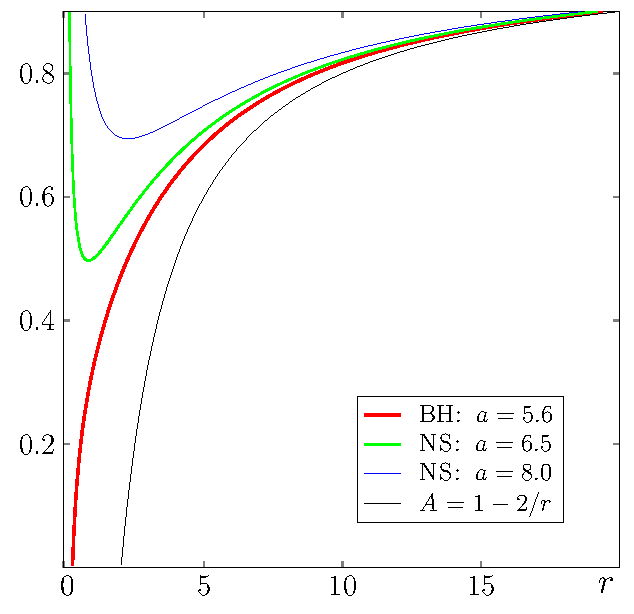
\includegraphics [width=0.483\textwidth]{Figure1}
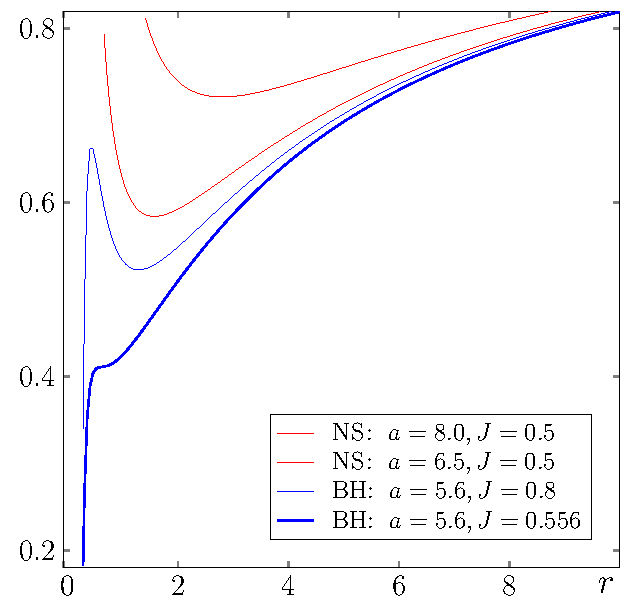
\includegraphics [width=0.483\textwidth]{Figure2}
\end{center}\vspace{-1ex}
\caption{1.\;Left: the metric functions $A(r)$ with the same mass ($M=1$). Right: the effective potentials of freely falling  particles.}
\label{fig1}
\end{figure}

\end{frame}

%##################  7  ###################
\begin{frame}
{\centerline {Tidal forces\quad}}

\begin{figure}[]
\begin{center}
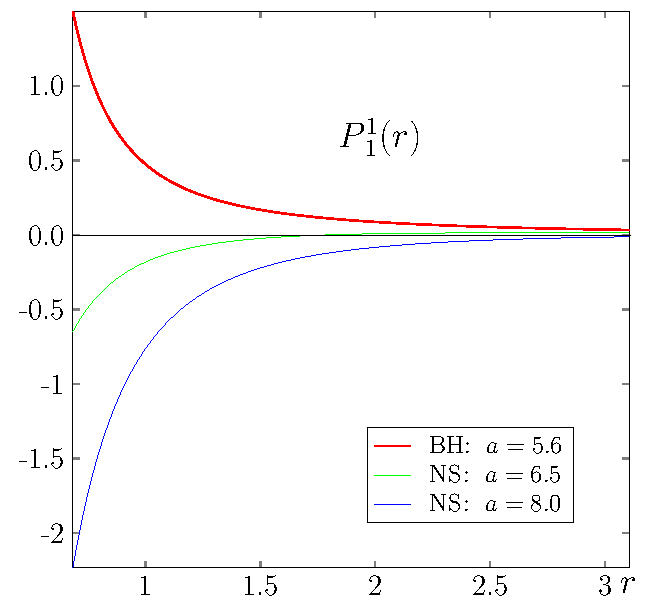
\includegraphics [width=0.483\textwidth]{Figure3}
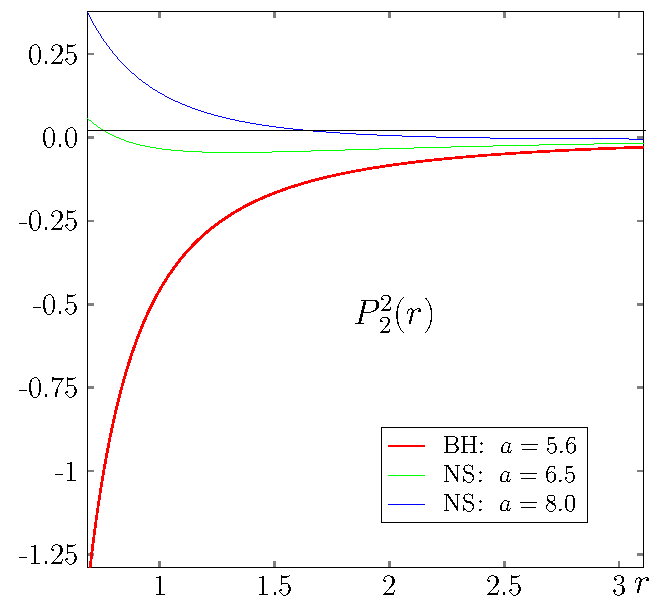
\includegraphics [width=0.483\textwidth]{Figure4}
\end{center}\vspace{-1ex}
\caption{2.\;Tidal forces: $F_t^{i}\equiv\dfrac{D^2\eta^{i}}{ds^2}= R^{i}_{jkl} U^{j}U^{k}\eta^{l} = P^{i}_{l}\eta^{l}$.}
\label{fig1}
\end{figure}

\end{frame}


%################  8  ###################
\begin{frame}
{\centerline{What happens when a star is destroyed}\\ \centerline{by a supermassive black hole?}\vspace{-3ex}}

\vspace{-1ex}
\begin{figure}[]
\begin{center}\hspace{-2em}
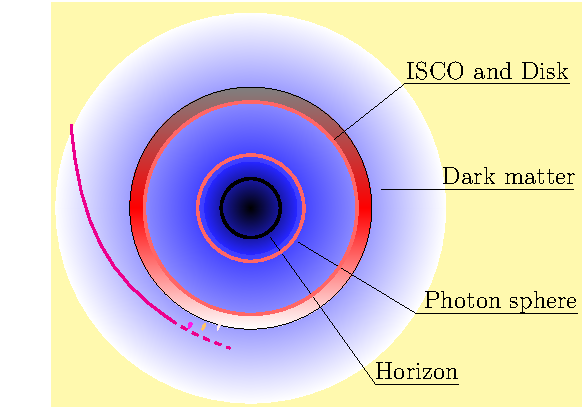
\includegraphics [width=0.65\textwidth]{Figure5}
\end{center}\vspace{-1ex}
\caption{3.\;The tidal disruption of a star near a BH. One part of the debris falls onto the accretion disk, while the other escapes from the pericenter.}
\label{fig3}
\end{figure}

\end{frame}


%##################  9  ###################
\begin{frame}
{\centerline{What happens when a star collides}\\ \centerline{with a shell of gray matter?}\vspace{-3ex}}

\vspace{-1ex}
\begin{figure}
\begin{center}\hspace{-2em}
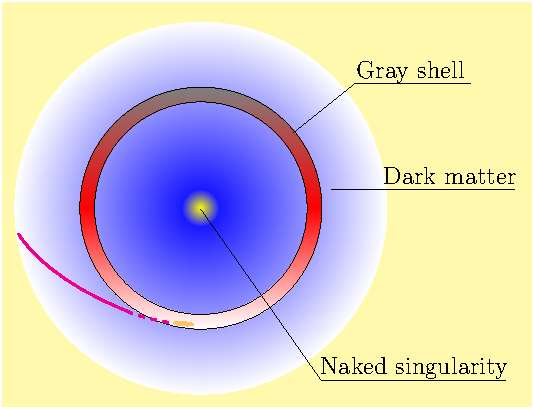
\includegraphics [width=0.62\textwidth]{Figure6}
\end{center}\vspace{-1ex}
\caption{4.\;The collision of a star having a small angular momentum with the gray shell formed by baryonic matter in the potential well.}
\end{figure}

\end{frame}

%##################  10  ###################
\begin{frame}
{\centerline{Conclusion}}

\vspace{4ex}\large{
Further observations of tidal disruption events will help us to distinguish between supermassive black holes and naked singularities in the centers of galaxies.}

\vspace{4ex}\Large{
\textcolor{blue}{\qquad\qquad Thank you for your attention!}}

\end{frame}



\end{document}


